% questions.tex -- Module 5 (Advanced Mechanics) short-answer booklet, HSC Section II style.
% 20 questions, 90 marks: Topic 1 Q1-6 (28 marks), Topic 2 Q7-13 (33), Topic 3 Q14-20 (29).
% Answers, marking criteria and sample answers: answers.tex.
% Every number: checks/m5-short-answer/numbers.py
% Build: TEXINPUTS=.: xelatex questions.tex (twice)
\documentclass[12pt]{article}
\usepackage{quiz}
\hypersetup{pdftitle={Short Answer Questions - Module 5 - Advanced Mechanics}}

\begin{document}
\quiztitle{Year 12 Physics}{Short Answer Questions - Module 5 - Advanced Mechanics}
\begin{center}
  20 questions \textperiodcentered\ 90 marks \textperiodcentered\ allow about 2 hours 40 minutes\\[2pt]
  Show all working. Use $g = \qty{9.8}{m.s^{-2}}$, $G = \qty{6.67e-11}{N.m^2.kg^{-2}}$,
  $M_\mathrm{E} = \qty{6.0e24}{kg}$, $r_\mathrm{E} = \qty{6.371e6}{m}$.
\end{center}

% =====================================================================
\firsttopictitle{Topic 1 - Projectile Motion}

% ---- Q1
\begin{saq}{4}
A golf ball is hit from level ground with a velocity of \qty{28}{m.s^{-1}} at \ang{35} above the
horizontal. Ignore air resistance.
\qpartL{a}{2}{Calculate the maximum height reached by the ball.}{5}
\qpartL{b}{2}{Calculate the horizontal range of the ball.}{5}
\end{saq}

% ---- Q2
\Needspace{30\baselineskip}
\begin{saq}{5}
A ball is thrown horizontally at \qty{15}{m.s^{-1}} from the top of a building \qty{30}{m} high. Ignore
air resistance.
\begin{center}
  \begin{tikzpicture}[x=0.8cm, y=0.8cm]
    \draw[line width=0.6pt] (-1.5,0) -- (6.5,0);
    \draw[fill=black!12] (-1.2,0) rectangle (0,3.2);
    \draw[->, line width=0.7pt] (0.15,3.35) -- (0.9,3.35) node[above, font=\small] {\qty{15}{m.s^{-1}}};
    \shade[ball color=black!25] (0.05,3.35) circle (0.12);
    \draw[guide, domain=0:4.4, samples=40, smooth] plot (\x, {3.35-3.35*(\x/4.4)^2});
    \draw[|<->|, line width=0.4pt] (-1.5,0) -- (-1.5,3.2) node[midway, left, font=\small] {\qty{30}{m}};
  \end{tikzpicture}
\end{center}
\qpartL{a}{2}{Calculate the time taken for the ball to reach the ground.}{4}
\qpartL{b}{3}{Calculate the velocity of the ball just before it hits the ground. Give its magnitude
and direction.}{7}
\end{saq}

% ---- Q3
\Needspace{98mm}
\begin{saq}{3}
A projectile is launched at an angle above the horizontal. Using Newton's laws of motion, explain
why the path of the projectile is a parabola. Ignore air resistance.
\alines{8}
\end{saq}

% ---- Q4
\Needspace{24\baselineskip}
\begin{saq}{4}
A ball is launched from level ground with speed $u$ at an angle $\theta$ above the horizontal. It
lands at the same height at time $T$. Ignore air resistance.

On the axes below, sketch graphs of the horizontal velocity $v_x$ and the vertical velocity $v_y$ of
the ball from launch until it lands. Take upwards as positive. Label the key features of each graph.
\begin{center}
  \begin{tikzpicture}
    \draw[axisline] (0,0) -- (5.2,0) node[right] {$t$};
    \draw[axisline] (0,-2.2) -- (0,2.4) node[above] {$v_x$};
    \node[left, font=\small] at (0,0) {0};
    \draw (4.4,0.08) -- (4.4,-0.08) node[below, font=\small] {$T$};
  \end{tikzpicture}\hspace{12mm}%
  \begin{tikzpicture}
    \draw[axisline] (0,0) -- (5.2,0) node[right] {$t$};
    \draw[axisline] (0,-2.2) -- (0,2.4) node[above] {$v_y$};
    \node[left, font=\small] at (0,0) {0};
    \draw (4.4,0.08) -- (4.4,-0.08) node[below, font=\small] {$T$};
  \end{tikzpicture}
\end{center}
\end{saq}

% ---- Q5 (practical investigation: range of a ball rolling off a bench)
\Needspace{40\baselineskip}
\begin{saq}{8}
A student investigates the motion of a ball that rolls off a horizontal bench of height
\qty{0.90}{m}. A light gate measures the launch speed $u$ of the ball as it leaves the bench. The
student measures the range $R$: the horizontal distance from the edge of the bench to where the
ball lands. The results are shown in the table.
\begin{center}
  \renewcommand\arraystretch{1.5}
  \begin{tabular}{|l|*{5}{>{\centering\arraybackslash}p{15mm}|}}
    \hline
    \textbf{Launch speed $u$ (\si{m.s^{-1}})} & 1.0 & 1.5 & 2.0 & 2.5 & 3.0\\ \hline
    \textbf{Range $R$ (\si{m})} & 0.43 & 0.63 & 0.87 & 1.06 & 1.29\\ \hline
  \end{tabular}
\end{center}
\qpart{a}{3}{On the grid below, plot the data and draw a line of best fit.}
\begin{center}
  \begin{tikzpicture}
    \begin{axis}[width=125mm, height=95mm, axis lines=left, xmin=0, xmax=3.5, ymin=0, ymax=1.6,
        xtick={0,0.5,...,3.5}, ytick={0,0.2,...,1.6}, minor x tick num=4, minor y tick num=3,
        grid=both, major grid style={black!45, line width=0.35pt},
        minor grid style={black!18, line width=0.25pt},
        tick label style={font=\small}, label style={font=\small},
        xticklabel style={/pgf/number format/fixed, /pgf/number format/fixed zerofill, /pgf/number format/precision=1},
        yticklabel style={/pgf/number format/fixed, /pgf/number format/fixed zerofill, /pgf/number format/precision=1},
        xlabel={Launch speed $u$ (\si{m.s^{-1}})}, ylabel={Range $R$ (\si{m})},
        scaled ticks=false, enlargelimits=false]
      \addplot[draw=none] coordinates {(0,0)};
    \end{axis}
  \end{tikzpicture}
\end{center}
\qpartL{b}{3}{Using the gradient of your line of best fit, determine a value for the acceleration due
to gravity, $g$.}{7}
\qpartL{c}{2}{Explain ONE way the student could improve the accuracy of the results.}{4}
\end{saq}

% ---- Q6 (launched upwards from a cliff)
\Needspace{140mm}
\begin{saq}{4}
A stone is thrown from the top of a cliff \qty{25}{m} high with a velocity of \qty{12}{m.s^{-1}} at
\ang{40} above the horizontal. It lands on flat ground at the base of the cliff. Ignore air
resistance.
\begin{center}
  \begin{tikzpicture}[x=0.8cm, y=0.8cm]
    \draw[line width=0.6pt] (-1.5,0) -- (4.2,0);
    \draw[fill=black!12] (-1.2,0) rectangle (0,2.5);
    \draw[->, line width=0.7pt] (0,2.5) -- ({0.9*cos(40)},{2.5+0.9*sin(40)}) node[above, font=\small] {\qty{12}{m.s^{-1}}};
    \draw ({0.45},2.5) arc (0:40:0.45); \node[font=\scriptsize] at (0.75,2.68) {\ang{40}};
    \draw[guide, domain=0:2.92, samples=50, smooth] plot (\x, {2.5 + 0.839*\x - 0.580*\x*\x});
    \draw[|<->|, line width=0.4pt] (-1.5,0) -- (-1.5,2.5) node[midway, left, font=\small] {\qty{25}{m}};
  \end{tikzpicture}
\end{center}
Calculate the horizontal distance from the base of the cliff to where the stone lands.
\alines{9}
\end{saq}

% =====================================================================
\topictitle{Topic 2 - Circular Motion}

% ---- Q7 (car on a flat bend)
\begin{saq}{3}
A car travels around a flat, horizontal bend at a constant speed.
\qpartL{a}{1}{Identify the force that provides the centripetal force on the car.}{2}
\qpartL{b}{2}{Explain why the car is more likely to skid if it goes around the bend at a higher
speed.}{5}
\end{saq}

% ---- Q8 (banked curve)
\Needspace{34\baselineskip}
\begin{saq}{7}
A car travels around a curve of radius $r$ that is banked at an angle $\theta$ to the horizontal. It
travels at the design speed $v$, so there is no sideways friction on the car.
\qpart{a}{2}{On the diagram, draw and label the forces acting on the car. Show the direction of the
net force.}
\begin{center}
  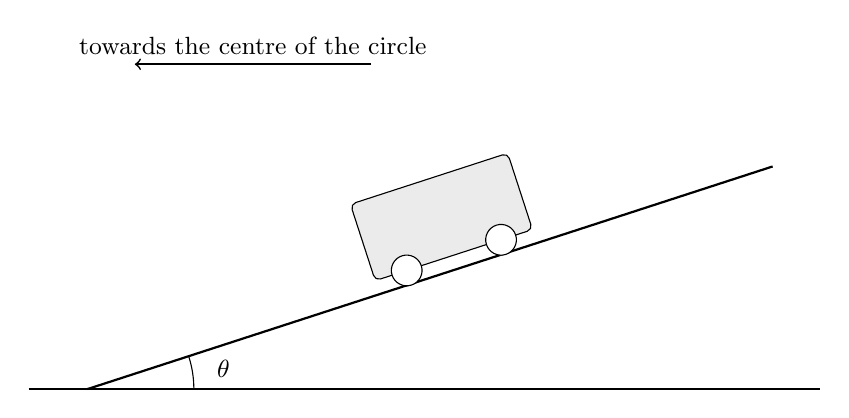
\begin{tikzpicture}[scale=1.5]
    \draw[line width=0.6pt] (-0.5,0) -- (6.2,0);
    \draw[line width=0.8pt] (0,0) -- (5.8,{5.8*tan(18)});
    \draw (0.9,0) arc (0:18:0.9); \node[font=\small] at (1.15,0.17) {$\theta$};
    \begin{scope}[shift={({3.3*cos(18)},{3.3*sin(18)})}, rotate=18]
      \draw[fill=black!8, rounded corners=2pt] (-0.7,0.12) rectangle (0.7,0.8);
      \draw[fill=white] (-0.42,0.12) circle (0.13); \draw[fill=white] (0.42,0.12) circle (0.13);
    \end{scope}
    \draw[->, line width=0.6pt] (2.4,2.75) -- (0.4,2.75) node[midway, above, font=\small] {towards the centre of the circle};
  \end{tikzpicture}
\end{center}
\qpartL{b}{3}{Show that the design speed is given by $\tan\theta = \dfrac{v^2}{rg}$.}{8}
\qpartL{c}{2}{A curve of radius \qty{80}{m} is banked at \ang{15}. Calculate its design speed.}{4}
\end{saq}

% ---- Q9 (conical pendulum)
\Needspace{30\baselineskip}
\begin{saq}{4}
A \qty{0.25}{kg} ball hangs from a string \qty{0.80}{m} long. The ball moves in a horizontal circle,
with the string at \ang{30} to the vertical.
\begin{center}
  \begin{tikzpicture}
    \draw[line width=1pt] (-0.8,3.2) -- (0.8,3.2); \fill[pattern=north east lines] (-0.8,3.2) rectangle (0.8,3.4);
    \draw[guide] (0,1.0) ellipse (1.2 and 0.28);
    \draw[guide] (0,3.2) -- (0,0.6);
    \draw[line width=0.7pt] (0,3.2) -- (1.2,1.0);
    \draw (0,2.7) arc (270:298.6:0.5); \node[font=\scriptsize] at (0.2,2.4) {\ang{30}};
    \node[right, font=\small] at (0.65,2.2) {\qty{0.80}{m}};
    \shade[ball color=black!20] (1.2,1.0) circle (0.14);
  \end{tikzpicture}
\end{center}
\qpartL{a}{2}{Calculate the tension in the string.}{5}
\qpartL{b}{2}{Calculate the speed of the ball.}{5}
\end{saq}

% ---- Q10 (vertical circle)
\Needspace{20\baselineskip}
\begin{saq}{4}
A \qty{0.20}{kg} ball on a string is swung in a vertical circle of radius \qty{0.60}{m}.
\qpartL{a}{2}{Calculate the minimum speed the ball must have at the top of the circle for the string to
stay tight.}{5}
\qpartL{b}{2}{At the bottom of the circle the ball moves at \qty{6.0}{m.s^{-1}}. Calculate the tension in
the string at this point.}{5}
\end{saq}

% ---- Q11 (torque on a wrench)
\Needspace{24\baselineskip}
\begin{saq}{5}
A mechanic pushes on the end of a wrench of length \qty{0.35}{m} with a force of \qty{150}{N}, at
\ang{70} to the handle.
\begin{center}
  \begin{tikzpicture}
    \draw[fill=black!15, rounded corners=2pt] (0,-0.1) rectangle (4,0.1);
    \draw[fill=white, line width=0.7pt] (0,0) circle (0.3); \node[font=\scriptsize] at (0,-0.55) {nut};
    \draw[force] (4,0) -- ++({1.2*cos(110)},{1.2*sin(110)}) node[above, font=\small] {\qty{150}{N}};
    \draw (3.55,0) arc (180:110:0.45); \node[font=\scriptsize] at ({4+0.75*cos(145)},{0.75*sin(145)}) {\ang{70}};
    \draw[|<->|, line width=0.4pt] (0,-0.9) -- (4,-0.9) node[midway, below, font=\small] {\qty{0.35}{m}};
  \end{tikzpicture}
\end{center}
\qpartL{a}{2}{Calculate the torque applied to the nut.}{4}
\qpartL{b}{1}{The nut needs a torque of \qty{65}{N.m} to loosen it. Calculate the smallest force that
would loosen the nut if it is applied at the end of the wrench.}{3}
\qpartL{c}{2}{The mechanic slides a pipe over the handle to make the wrench longer. Explain why this
makes it easier to loosen the nut.}{5}
\end{saq}

% ---- Q12 (practical investigation: centripetal force)
% Data: r = 0.60 m, v^2 = 16 ... 64 m^2/s^2, F = 0.82 ... 3.18 N; best-fit gradient 0.050 kg/m.
\Needspace{40\baselineskip}
\begin{saq}{7}
A student uses the apparatus shown to investigate centripetal force. The hanging masses provide the
centripetal force $F$ on the rubber stopper. The radius of the circle is kept at \qty{0.60}{m}. For
each value of $F$, the student finds the speed $v$ of the stopper by timing 10 revolutions. Assume the
string to the stopper stays horizontal.
\begin{center}
  \begin{tikzpicture}
    \draw[guide] (0,2.6) ellipse (1.8 and 0.35);
    \draw[fill=black!8] (-0.08,0.9) rectangle (0.08,2.6);
    \draw[line width=0.7pt] (0,2.6) -- (1.75,2.6); \draw[fill=black!40] (1.75,2.48) rectangle (1.98,2.72);
    \draw[line width=0.7pt] (0,0.9) -- (0,0.55); \draw[fill=black!40] (-0.18,0.2) rectangle (0.18,0.55);
    \node[right, font=\small] at (2.0,2.6) {Rubber stopper};
    \node[right, font=\small] at (0.25,0.38) {Hanging masses};
    \node[right, font=\small] at (0.15,1.6) {Glass tube};
    \draw[|<->|, line width=0.4pt] (0,2.95) -- (1.86,2.95) node[midway, above, font=\small] {\qty{0.60}{m}};
  \end{tikzpicture}
\end{center}
The graph shows the results.
\begin{center}
  \begin{tikzpicture}
    \begin{axis}[width=120mm, height=80mm, axis lines=left, xmin=0, xmax=70, ymin=0, ymax=3.5,
        xtick={0,10,...,70}, ytick={0,0.5,...,3.5}, minor x tick num=1, minor y tick num=4,
        grid=both, major grid style={black!40, line width=0.3pt}, minor grid style={black!15, line width=0.2pt},
        tick label style={font=\small}, label style={font=\small},
        yticklabel style={/pgf/number format/fixed, /pgf/number format/fixed zerofill, /pgf/number format/precision=1},
        xlabel={$v^2$ (\si{m^2.s^{-2}})}, ylabel={Centripetal force $F$ (\si{N})},
        scaled ticks=false, enlargelimits=false]
      \addplot[only marks, mark=*, mark size=2pt] coordinates {(16,0.82) (25,1.24) (36,1.78) (49,2.47) (64,3.18)};
      \addplot[line width=0.8pt, domain=0:68] {0.050*x};
    \end{axis}
  \end{tikzpicture}
\end{center}
\qpartL{a}{2}{Explain why the student plotted $F$ against $v^2$, rather than $F$ against $v$.}{4}
\qpartL{b}{3}{Use the graph to determine the mass of the rubber stopper.}{6}
\qpartL{c}{2}{Explain why timing 10 revolutions gives a more accurate value of $v$ than timing one
revolution.}{4}
\end{saq}

% ---- Q13 (kinetic energy in uniform circular motion)
\Needspace{92mm}
\begin{saq}{3}
An object moves in uniform circular motion. Explain why its kinetic energy stays constant even
though a net force acts on it.
\alines{7}
\end{saq}

% =====================================================================
\topictitle{Topic 3 - Motion in Gravitational Fields}

% ---- Q14 (g on Mars)
\begin{saq}{3}
Mars has a mass of \qty{6.42e23}{kg} and a radius of \qty{3.39e6}{m}.
\qpartL{a}{2}{Calculate the gravitational field strength at the surface of Mars.}{4}
\qpartL{b}{1}{Calculate the weight of a \qty{70}{kg} astronaut standing on the surface of Mars.}{2}
\end{saq}

% ---- Q15 (derive Kepler's third law; geostationary radius)
\Needspace{24\baselineskip}
\begin{saq}{5}
\qpartL{a}{3}{A satellite of mass $m$ moves in a circular orbit of radius $r$ around a planet of mass
$M$, with period $T$. Derive the relationship $\dfrac{r^3}{T^2} = \dfrac{GM}{4\pi^2}$.}{8}
\qpartL{b}{2}{Calculate the orbital radius of a geostationary satellite around Earth (period
24.0 hours).}{5}
\end{saq}

% ---- Q16 (compare LEO and GEO)
\Needspace{120mm}
\begin{saq}{4}
Compare the orbit of a low Earth orbit (LEO) satellite with the orbit of a geostationary (GEO)
satellite. In your answer, refer to their altitude, orbital speed and period, and give one use of
each type of satellite.
\alines{10}
\end{saq}

% ---- Q17 (energy changes between orbits)
\Needspace{24\baselineskip}
\begin{saq}{5}
A \qty{500}{kg} satellite is moved from a circular orbit of radius \qty{7.0e6}{m} to a circular orbit of
radius \qty{1.4e7}{m} around Earth.
\qpartL{a}{2}{Calculate the change in the gravitational potential energy of the satellite.}{5}
\qpartL{b}{2}{Calculate the change in the kinetic energy of the satellite.}{5}
\qpartL{c}{1}{Hence, determine the minimum energy that the rocket engines must supply.}{2}
\end{saq}

% ---- Q18 (escape velocity)
\Needspace{20\baselineskip}
\begin{saq}{4}
\qpartL{a}{3}{Using the law of conservation of energy, show that the escape velocity from the surface
of a planet of mass $M$ and radius $r$ is $v_\mathrm{esc} = \sqrt{\dfrac{2GM}{r}}$.}{8}
\qpartL{b}{1}{Calculate the escape velocity from the surface of Mars ($M = \qty{6.42e23}{kg}$,
$r = \qty{3.39e6}{m}$).}{2}
\end{saq}

% ---- Q19 (comet: fastest when closest)
\Needspace{92mm}
\begin{saq}{3}
A comet moves in an elliptical orbit around the Sun. Using the law of conservation of energy,
explain why the comet moves fastest when it is closest to the Sun.
\alines{7}
\end{saq}

% ---- Q20 (evaluate: no gravity on the ISS)
\Needspace{142mm}
\begin{saq}{5}
A student says: \emph{\textquotedblleft Astronauts on the International Space Station (ISS) float
because there is no gravity in space.\textquotedblright}

The ISS orbits Earth at an altitude of \qty{420}{km}. Evaluate the student's statement. Support your
answer with a calculation.
\alines{12}
\end{saq}

\end{document}
